%\documentclass[UTF8]{ctexart} % use larger type; default would be 10pt
\documentclass[a4paper]{article}
\usepackage{hw}

%ASSP
\DeclareMathOperator{\tb}{\text{TB}}
\DeclareMathOperator{\MF}{\text{MF}}

\newcommand{\dis}{\displaystyle}
\numberwithin{equation}{section}

\title{固体理论, Homework 09}
\author{王石嵘 20110220098}
\date{\today} % Activate to display a given date or no date (if empty),
         % otherwise the current date is printed 

\begin{document}
% \boldmath
\maketitle

%\tableofcontents

%\newpage

%\setcounter{section}{-1}

\section{考虑一个正方晶格上的单带模型:}

\begin{equation}\label{key}
	H= \sum_k(\epsilon_k-\mu)c_k^\dagger c_k + V\sum_i n_i n_{i+\hat x}
\end{equation}
这里第二项是$ x $方向上最近邻电子之间的排斥相互作用。我们假设该系统在零温下形成了一个$ x $方向的自旋密度波序,序参量为
\begin{equation}\label{key}
	\phi = (-1)^{i_x}n_i
\end{equation}
其中$ i_x $指格点$ i $的$ x $坐标,$ n_i=c_i^\dagger c_i $为电子密度算符。在计算中,可以取晶格常数为单位1。

\begin{enumerate}
\item
证明
\begin{equation}\label{key}
	\phi = \frac1N \sum_k c_k^\dagger c_{k+Q}
\end{equation}
这里$ Q=(\pi,0) $,$ N $为总格点数。(提示:假设对于电荷密度波序,$ \phi $是与位置$ i $无关的常数。)
\item 对上面的哈密顿量进行平均场分解并求出准粒子激发的能谱。
\item 定性描述在产生电荷密度波序前后体系费米面的变化(可以用示意图表示)。
这里假设$ \epsilon_k=k^2/2m $,并且费米面的直径大于$ \pi $。
\item 在零温时推导序参量的自洽方程。(注:可以保留对$ k $的积分或者求和,不用积出来。)

\end{enumerate}

\paragraph{Solution:}
\subparagraph{1.}
~\vspace{70pt}\\
\subparagraph{2.}
Let $ \Delta = 2V\delta n $, $ \xi_k = \epsilon_k - \mu $
\begin{equation}\label{key}
	H^{\MF} = \sum_k (\xi_k) c_k^\dagger c_k - \Delta \sum_k  \sum_k c_k^\dagger c_{k+Q}
\end{equation}
\begin{equation}\label{key}
	H^{\MF} = \sum_k \mqty(c_k^\dagger & c_{k+Q}^\dagger) 
		\mqty(\xi_k & -\Delta\\ - \Delta & \xi_{k+Q} ) 
		\mqty(c_k \\ c_{k+Q}) 
\end{equation}
\begin{equation}\label{key}
	E_k = \dfrac{\xi_k + \xi_{k+Q}}{2} \pm \sqrt{\qty( \dfrac{\xi_k - \xi_{k+Q}}{2} )^2 + \Delta^2}
\end{equation}
In case $ \xi_k = \xi_{k+Q} $
\begin{equation}\label{key}
	E_k = \xi_k \pm \Delta
\end{equation}
\newpage
\subparagraph{3.}~\\
\begin{figure}[H]
	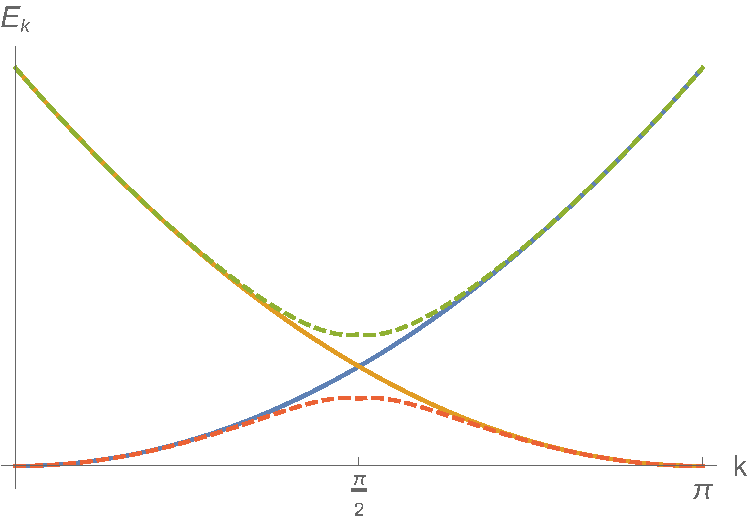
\includegraphics[width=0.6\linewidth]{Ek.pdf}
\end{figure}
Dashed: after CDW.

\subparagraph{4.}

\end{document}